%
% proposal.tex
%
% Dissertation Proposal Template.
% School of Computing
% Clemson University
%
\documentclass[10pt]{ClemsonProposal}

\usepackage{caption,subcaption}
\usepackage{graphicx}
% This is nice for source code listings
\usepackage{listings}
\usepackage{tabularx}

% This is needed to include figures
% \usepackage{graphicx}

% Use any additional packages you might need


%
% Give values to the variables used in this document
%
\title{Galois for FPGA\\An Efficient Microarchitecture and Compiler for Accelerating Amorphous Data Parallel Graph Applications}
\department{Department of Electrical and Computer Engineering}
\university{The University of Texas at Austin}
\documenttype{Dissertation Proposal}
\major{Computer Architecture and Embedded Processors}
\proposalday{20}
\proposalmonth{April}
\proposalyear{2015}
\author{Dan Zhang}
\committeechair{Keshav Pingali}
\committeememberone{Derek Chiou}
\committeemembertwo{Mattan Erez}
\committeememberthree{Andreas Gerstlauer}
\committeememberfour{Eric Chung}

% Just in case you have more then 3 committee members
% \committeememberfive{Member5 Name}
% \committeemembersix{Member6 Name}


%
% PDF Setup -- You should not need to change this
%
\hypersetup{
    colorlinks,
    linkcolor={black},
    citecolor={black},
    filecolor={black},
    urlcolor={black},
    pdftitle={\thetitle},
    pdfauthor={\theauthor},
    pdfsubject={\thedocumenttype},
    pdfkeywords={The University of Texas at Austin, \theauthor, \thedocumenttype},
    pdfstartpage={1}
}


%
% User-specified command definitions/redefinitions
%
\newcommand{\cplusplus}{{\rm C\raise.5ex\hbox{\small ++}}}


\begin{document}
%   ==========================================================================
%   Begin front matter (pages are numbered with roman numerals)
%   ==========================================================================
    \begin{frontmatter}
        \maketitle
		\tableofcontents
        \newpage

        % Generate the abstract
        %!TEX root = proposal.tex
\begin{abstract}

Although the behavior of irregular algorithms can be very complex, many of them have a generalized form of data 
parallelism known as \textit{amorphous data parallelism}. Through the use of unordered atomic transactions and 
dynamic worklist-based scheduling, the Galois system has been demonstrated to be a practical approach to exploiting 
this form of parallelism. I propose Galois for FPGA, an efficient custom microarchitecture and compiler to run 
Galois programs at higher performance and power efficiency than traditional general-purpose architectures.

\end{abstract}

	\end{frontmatter}



%   ==========================================================================
%   Begin main matter (pages are numbered with arabic numerals)
%   ==========================================================================
    \doublespacing     % Text should be double spaced
    \pagestyle{fancy}  % Turn the nice header on for the rest of the document

    %
    % I use a file for every section.  Each of these corresponds to a file
    % with the specified name ending in '.tex' (e.g., introduction.tex).
    %
    %!TEX root = proposal.tex
%\addbibresource{bibliography.bib}
%----------------------------------------------------------------------------
\section{Introduction}\label{sect:problem}
%----------------------------------------------------------------------------

The pervasiveness of multicore processors have shifted the burden of improving program execution speed from chip 
manufacturers to software developers. Data parallelism often occurs in \textit{regular} programs, which manipulate 
dense matrices and arrays. Many language constructs have been proposed to enable programmers to easily express 
regular data-parallel application in their apps, such as parallel-for in OpenMP \cite{openmpScheduling}, thread 
blocks in CUDA \cite{cuda}, and work-groups in OpenCL \cite{opencl}.

However, \textit{irregular} programs are much harder to parallelize. Irregular programs use pointer-based data 
structures such as lists, trees, and graphs, and are common outside of computational science. Examples can be found 
in domains like n-body simulation \cite{barneshut}, data mining \cite{datamining}, 
maxflow \cite{cormen}, social networks \cite{communityDiscovery}, 
and meshing \cite{dmr}. Recent research efforts have made considerable headway, demonstrating that data-driven 
parallel algorithms are algorithmically efficient and support higher performance than topology-driven 
implementations on both general purpose processors \cite{galoisVsVertex} \cite{thinkLikeVertex} as well as GPUs 
\cite{galoisGPU} \cite{datavstopGPU}.

One system for data-driven applications is Galois \cite{galois}, which comprises the Galois worklist-based 
data-driven programming model, the unordered transactional \textbf{foreach} iterator, a set of concurrent library 
components, and the Galois software runtime system. These applications can benefit significantly from dedicated 
worklist accelerators on both general purpose multicore processors \cite{carbon} and GPUs \cite{gpuWorklist}. 
However, as fixed logic, these accelerators cannot be easily adapted to the different scheduling requirements of 
each algorithm, potentially resulting in lost performance \cite{galoisOrdering}.


%----------------------------------------------------------------------------
\subsection{Thesis Proposal}
%----------------------------------------------------------------------------

For my thesis, I propose the Galois system for FPGA, consisting of a microarchitecture designed to accelerate 
Galois applications, a set of hardware accelerators matching the Galois software library components, and a compiler 
to emit a custom pipelined engine from Galois software code. By automatically generating custom hardware from a 
Galois software specification, Galois for FPGA can achieve both higher performance and energy efficiency compared to 
Galois running on general purpose hardware.


\subsection{The Galois System}


\begin{figure}
\centering
\lstset{language=Java}
\begin{lstlisting}
Graph graph = { /* init */}; // Initialize graph contents
WorkList<GraphNode> workQ();
workQ.enq(init); // worklist initialized with the starting node
foreach(uint nid : workQ) {
   uint nid = workQ.deq();
   GraphNode node = graph.getNode(nid);
   for(int i = 0; i < node.numEdges; i++) {
      Edge e = graph.getEdge(node.edgePtr + i);
      uint newDist = node.dist + edge.weight;
      if(newDist < graph.getNode(edge.dest).dist) {
         node.dist = newDist;
         workQ.enq(edge.dest);
      }
   }
}
\end{lstlisting}
\caption{Galois pseudocode for SSSP}
\label{fig:ssspSource}
\end{figure}

In \cite{galois}, Pingali et al. introduce the notion of operator formulation, in which an algorithm is viewed in 
terms of its action on data structures. The authors demonstrate that operator formulation is both general 
\cite{galoisAlgorithms} and effectively exposes the fine-grained amorphous data-parallelism present in irregular 
algorithms \cite{galoisPerf}. They 
propose the Galois programming model, which is a sequential, object-oriented model that is augmented with the 
Galois set operator \textbf{foreach(e in Set S) \{B(e)\}}, in which the loop body \textit{B(e)} is executed for each 
element \textit{e} of set \textit{S}. Set \textit{S} may be either partially ordered or unordered. However, unlike 
a regular \textbf{for} loop, the loop ordering is treated as a hint simply to improve performance. It is the 
programmer's responsibility to write Galois code in a way that ordering does not affect algorithm correctness. Each 
loop iteration may conflict with one another. The Galois runtime automatically generates locking mechanisms to 
ensure atomicity is not violated. When an iteration 
executes, it may add additional elements to set \textit{S}. In Galois, set \textit{S} is referred to as the 
\textbf{\textit{worklist}}.

The Galois system provides a concurrent data structure library, including worklists and graphs. Each data structure 
has several variants, each with several parameters; it's up to the programmer to choose the best variant and 
parameters to fit the algorithm and input. However, with a properly designed algorithm, the variant chosen only 
affects performance, not correctness.

\subsubsection{SSSP on Galois}

As a simple example, consider Single-Source Shortest Path (SSSP), the problem of finding the shortest path from a 
single source node to all connected nodes. SSSP is a well-known and long-studied problem with many practical 
applications on a wide spectrum of graph types. The traditional serial approach to SSSP is Dijkstra's Algorithm 
\cite{dijkstra}, which uses a priority queue to process the node with the shortest cumulative distance from the 
single source node first. While this is an efficient serial algorithm \textit{(O(v log v + e))}, it is poorly 
suited for multithreading. Bellman-Ford \cite{bellmanford} trades off work efficiency \textit{(O(ev))} for 
parallelism by processing every edge connection in the graph until the distances converge. A more flexible 
solution is Delta-stepping \cite{deltaStepping}, which is a hybrid of Dijkstra's and Bellman-Ford. Rather than 
considering the vertex with the lowest distance like Dijkstra's, delta-stepping groups vertices into buckets. Within 
each bucket, vertices are unordered and thus can be executed in parallel. If the bucket size is 1, then 
delta-stepping is identical to Dijkstra's algorithm. If the bucket size is infinite, then delta-stepping is the same 
as Bellman-Ford. Thus, by choosing a proper bucket size, or delta, we can make the proper tradeoff between 
available parallelism and work efficiency. Note that the appropriate bucket size not only changes based on the graph 
input but also on the host architecture running the algorithm. Galois source code for SSSP is shown in Figure 
\ref{fig:ssspSource}. If the worklist \textit{workQ} is using strict priority order, then the source code is an 
implementation of Dijkstra's Algorithm. Else, the source code depicts delta-stepping.

\subsubsection{Galois vs. other programming models}

Galois contains a high-level programming model; thus it can be implemented within any parallel framework such as CUDA 
and OpenCL. The Galois authors have implemented Galois on both Java and C++, and are working towards implementing 
Galois for GPU using CUDA \cite{galoisGPU}. Davidson et al. \cite{gpuSSSP} demonstrated the potential value of Galois 
for GPU by implementing a SSSP delta-stepping within CUDA using worklists, claiming 14x to 340x higher performance 
compared to a Bellman-Ford implementation depending on the input. However, the authors had to construct custom 
Galois-like worklists and synchronization mechanisms on top of CUDA. As this was a custom solution designed to run 
only SSSP, these modules must be reimplemented to effectively target a different application. 
Considerable work must be done to build up the synchronization, scheduling, work-balancing, and 
work spilling features of a Galois worklist.


There are many other programming frameworks targeting graph applications, such as PowerGraph \cite{powergraph}, Ligra 
\cite{ligra}, and GraphGen \cite{graphgen}. These frameworks are all \textit{vertex-centric}, meaning that computation 
is expressed in terms of each vertex and its neighbors. The schedule is simple: iterate across all vertices in the 
graph until the algorithm converges. Although this programming model is useful and easy to understand, vertex-centric 
models can be inefficent since even nodes without any work must be executed every cycle. In addition, since a 
vertex only has information about its immediate neighbors, information is propogated slowly, 
one hop at a time. For example, Tian et al. \cite{thinkLikeVertex} demonstrated that a graph-centric model of a 
connected components algorithm ran 63x faster and used 204x fewer network messages than its vertex-centric 
counterpart. Its important to note that its possible to write vertex-centric programs within Galois \cite{galoisPerf}; 
however, Galois provides the user the flexibility to design more efficient graph-centric algorithms.

\subsection{Task Scheduling}

One common parallel programming approach is to decompose a program into parallel tasks and allow an underlying 
software layer to schedule these tasks to different threads. Examples of popular multithreaded task-based runtime 
systems include Cilk \cite{cilk}, OpenMP \cite{openmpScheduling}, and CUDA \cite{cuda}. These systems all implement 
sophisticated forms of load balancing, including techniques such as work stealing and chunking. However, researchers 
have demonstrated that many algorithms also benefit significantly proper task prioritization due to faster 
convergence, leading to a drastic net reduction in work \cite{gpuSSSP} \cite{adm}. State-of-the-art runtime systems 
like that in Galois are able to take advantage of this prioritization to achieve massive speedups 
\cite{galoisOrdering}.

Despite software tasked-based runtime systems already achieving a high degree of speedup, there is still room for even 
more improvement through hardware acceleration. Traditional multicore processors are not well suited towards executing 
parallel programs with abundant fine-grained parallelism expressed as many small threads \cite{isonet}. These programs 
have small tasks for which software task schedulers achieve only limited parallel speedups due to the increased 
overhead relative to the amount of work done per task \cite{carbon}. Researchers have proposed augmenting processors 
with dedicated hardware to aid in dynamic load distribution and balancing. Rigel is a 1024 core architecture designed 
for task-level parallelism through its task-centric memory model \cite{rigel}. StarT \cite{starT} implemented 
dedicated hardware queues for message passing with high priority levels for kernel code. Carbon \cite{carbon} proposes adding 
specialized instructions and dedicated hardware queues with fixed LIFO priority to handle task queue management. 
IsoNet \cite{isonet} proposes a dedicated network of load balancing engines scalable to thousands of cores. Dedicated 
hardware queues have even been proposed for GPUs \cite{gpuWorklist}. However, these techniques do not consider the 
potential performance improvements gained by a more optimal priority schedule. Although \cite{adm} proposes 
asynchronous direct messages to accelerate custom software schedulers, the authors only consider simple schedules such 
as FIFO and LIFO rather than true priority schedules.

Task scheduling is a first-order concern in the realm of internet core routers \cite{routerQoS}. State-of-the-art 
routers have the ability to dynamically schedule between tens of thousands of queues at hundreds of millions of 
scheduling decisions per second per chip \cite{router1tbps}. While there are differences between networking and 
fine-grained task scheduling, such as the size of the packets, latency timescales, and various other area and 
performance tradeoffs, some networking routing, prioritization, and scheduling algorithms may be relevant to my 
thesis. For my thesis, aside from developing my own worklist scheduling algorithms, I will consider scheduling 
techniques from networking to determine what concepts can be directly applied to improve my own scheduling techniques.

    %!TEX root = proposal.tex
%\addbibresource{bibliography.bib}
%-----------------------------------------------------------------------------
\section{Proposed Work}\label{sect:proposedWork}
%-----------------------------------------------------------------------------


%----------------------------------------------------------------------------
\subsection{Approach}
%----------------------------------------------------------------------------

The use of a high-level language like Galois with dynamic work generation and dynamic dependencies means that 
static scheduling approaches found in traditional high-level synthesis no longer apply. The Galois programming model semantics coupled with the 
Galois concurrent library components means that the user does not deal with issues such as atomicity, 
scheduling, work balancing, worklist spilling, prefetching, and more. In addition, the Galois HLS compiler is responsible for the 
generation of custom pipelines. These pipelines are multithreaded, in which each pipeline stage is working 
on a different thread. Unlike pipelines generated by traditional HLS tools such as Vivado, instructions flowing 
through the pipeline are issued dynamically as work items arrive. Pipeline stages may stall based on the control 
flow and variable latency accelerators. The compiler is responsible for generating the proper stall and forwarding 
logic to preserve correctness.

Due to pointer-chasing memory patterns and large memory footprint of graph applications, traditional memory 
hierarchies found in general purpose processors tend to perform poorly. This is where FPGAs can be much more effective. 
By tailoring the Galois microarchitecture to be able to saturate the available memory bandwidth of the system, an FPGA 
platform can outperform a general purpose CPU platform with similar bandwidth since the CPU often cannot effecitvely 
exploit all the available bandwidth in the system.

While the Galois for FPGA framework requires a substantial amount of work implementing transactional memory semantics, 
this is outside the scope of my thesis. My labmate Xiaoyu Ma will be implementing this as part of his thesis.


\subsection{Proposed User Workflow}

Using Galois for FPGA is similar to using Galois for software. The user writes a Galois program using the Galois library modes 
and the \textbf{foreach} Galois construct. This Galois program will have different syntax to the current Galois SW 
implementation in C++, but that's because the authors of Galois did not wish to implement a compiler, instead 
implementing Galois as several libraries within C++. In addition, instead of using C++, the Galois HLS compiler will use C 
and have the same restrictions as a standard HLS tool such as the lack of dynamic memory allocation outside of the 
Galois constructs, as I plan on implementing Galois by augmenting an existing HLS tool. Pragmas to provide high-level 
microarchitectural hints may be required, but will be avoided if possible.

After writing the Galois program, the user calls the Galois HLS compiler. The compiler generates the custom 
multithreaded pipelined engine code executing the \textbf{foreach} block and connects the engines to the Galois 
microarchitecture implemented in Bluespec. Parameters are passed to the Galois microarchitecture by the compiler with 
possible user input. Either the user or the compiler will tweak the parameters until the design meets timing and 
routing FPGA constraints.

\subsection{Galois Microarchitecture}

\begin{figure}
\centering
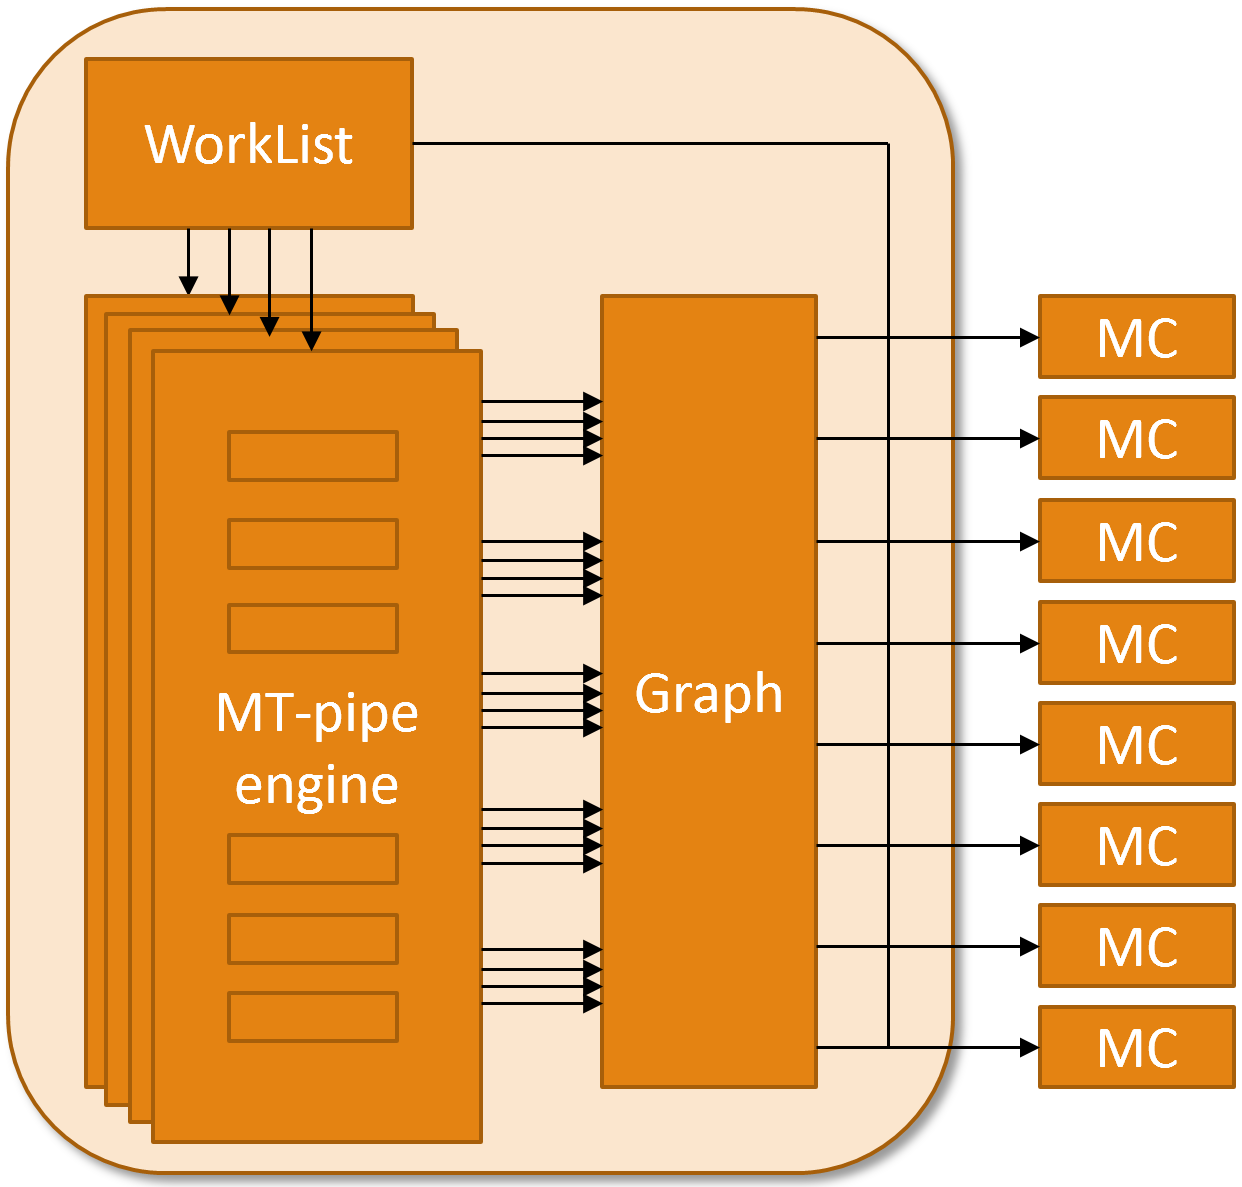
\includegraphics[width=6.5cm, keepaspectratio]{pics/uarch.png}
\caption{The Galois microarchitecture}
\label{fig:uarch}
\end{figure}

The Galois microarchitecture is a high-throughput packet processor that interfaces with custom engine code generated 
by the Galois HLS compiler as seen in Figure \ref{fig:uarch}. It consists of four major components: the custom engine code, the 
instantiated worklist, the instantiated graph module, and the surrounding infrastructure logic. The worklist and graph 
module variant and parameters are chosen by the user through explicit instantiation in the user code. Some other 
parameters may be set by the Galois HLS compiler based on the number of engines generated and the Galois library calls 
made by the engines. The surrounding infrastructure logic provides glue logic for the components and is custom to the 
target FPGA platform.

The Galois microarchitecture bears many similarities to Tera \cite{tera}. Like Tera, the Galois microarchitecture is 
a heavily multithreaded throughput system without data caches. However, there are several key differences. Since the 
Galois engines are custom-generated for the target program, they can achieve a high throughput per engine at low power. 
Depending on the application and available bandwidth in the FPGA platform, instead of 
needing 256 cores like Tera, the Galois microarchitecture only needs tens of engines or even fewer to fully saturate 
memory bandwidth. In addition, Galois supports a dedicated hardware priority scheduler and transactional memory 
framework.

\subsubsection{Worklist}

\begin{table}
\begin{tabular}{ | l | l | }
  \hline
  \textbf{Method} & \textbf{Description} \\
  \hline
  void enq(WorkItem work) & Enqueue work item into worklist \\
  \hline
  void enq(Priority p, WorkItem work) & Enqueue work item into worklist with priority p\\
  \hline
  WorkItem deq() & Dequeue and return work item from worklist \\
  \hline
\end{tabular}
\caption{Worklist interface}
\label{table:worklist}
\end{table}

The worklist library component performs work scheduling within the Galois microarchitecture. In the Galois programming 
model, the user writes a Galois kernel consisting of a foreach loop, wherein each loop iteration dequeues a work item 
from the worklist and may enqueue any number of additional work items to the worklist. The worklist therefore presents 
a simple FIFO interface is exposed to the programmer shown in Table \ref{table:worklist}, but behind the curtains it 
must perform dynamic work scheduling across tens to hundreds of threads on multiple engines across multiple FPGAs. In 
addition, the size of the worklist is unbounded, so the worklist must support dynamic fills and spills to memory. 
Proper care must be taken to ensure that work is balanced evenly using optimizations like work stealing, with 
optimizations such as streaming and double buffering to ensure memory spills and fills do not bottleneck the engines.

The standard worklist supports a simple FIFO schedule. However, many algorithms such as SSSP converge much faster 
given a priority schedule \cite{galoisOrdering}. Current state-of-the-art for software worklists require the user to 
specify a static priority algorithm, such as the bucket size for SSSP. Various priorities have been proposed for 
different algorithms, optimizing not only for convergence speed but also cache hit rate. Unfortunately, the best 
priority not only depends on the algorithm but also on the host architecture and shape of the input graph. In 
addition, I strongly suspect that the optimal priority may change as the amount of parallelism in the system 
dynamically grows and shrinks during execution.

\subsubsection{Worklist priority scheduling}

To further improve work efficiency, I propose the use of dynamic priority scheduling. Dynamic priority scheduling will 
utilize microarchitectural performance counters to optimize for convergence speed when possible. For example, in SSSP 
delta-stepping, the size of the bucket should be as small as possible while still providing enough work to avoid 
backpressuring the engines. By monitoring the amount of work in each bucket and the rate of engine work consumption, the 
worklist can dynamically adjust bucket size to provide near-optimal performance.

Other algorithms will require different types of scheduling to maximize the rate of convergence. Ideally, choosing the 
correct schedule should be determined by the microarchitecture. I will explore the possibility of determining the right 
scheduling algorithm to use and its parameters to maximize for performance, 
which is a function of the convergence rate and rate of work item completion.

\subsubsection{Graph}

\begin{table}
\begin{tabular}{ | l | l | }
  \hline
  \textbf{Method} & \textbf{Description} \\
  \hline
  void startTransaction() & Start atomic transaction \\
  \hline
  void endTransaction() & End atomic transaction \\
  \hline
  Node readNode(NodeID id) & Read node from graph \\
  \hline
  Edge readEdge(EdgeID id) & Read edge from graph \\
  \hline
  EdgeIterator readEdges(Node node) & Galois iterator for each edge in graph node\\
  \hline
  Bool cas(Payload\& cmpVal, Payload swapVal) & Compare-and-swap, returns success and old val\\
  \hline
  void writeNodePayload(Payload p) & Write node payload \\
  \hline
  void writeEdgePayload(Payload p) & Write edge payload \\
  \hline
\end{tabular}
\caption{Graph interface}
\label{table:graph}
\end{table}

Compiler-emitted Galois kernel engines do not interface directly with memory. Instead, they interface with the Graph 
concurrent library module, which handles preserving atomicity, interfacing with the underlying host memory fabric, and 
handling multiple memory operations in flight across multiple memory channels. The graph interface is shown in Table 
\ref{table:graph}. Note that the user will not have to explicitly call startTransaction() and endTransaction(). 
Instead, the Galois HLS compiler will emit these operations in place of the user. However, if the user wishes to 
perform low-level optimizations, he or she may choose to forgo the use of transactional memory and instead manually 
call the provided compare-and-swap atomic operation.

Note that this graph library module provided is a local computation graph, i.e. the graph structure does not change. 
The user is only able to modify the node payload contents, i.e. the local data associated with each node. This 
limitation still supports large number of graph algorithms, including SSSP, breadth-first search, preflow push, 
PageRank, and many more. I will investigate supporting mutable graphs using a simple hardware memory allocator and 
garbage collector.

\subsubsection{Galois Infrastructure}

The Galois infrastructure consists of glue logic, buffering, and flow control for the engines, worklist, and graph. 
Graph and worklist operations must be converted from generic memory operations to the interface required for running 
on that particular FPGA platform. Arbitration is required between the worklist and graph, as well as with the parallel 
workers within the worklist and graphs themselves. The infrastructure must balance requests between the available 
memory channels on the host and guarantee forward progress, as well as performance optimizations such as memory 
request balancing (either static or dynamic) across the memory channels. As each FPGA platform has its own unique 
memory interface, a new Galois infrastructure must be designed for every FPGA platform. The current infrastructure is 
designed to exploit the Convey MX-100 platform's atomic memory operations and multi-FPGA environment, 
which many platforms do not support.



\subsection{Galois HLS compiler}

For my thesis, I plan on augmenting an existing HLS compiler to support the \textbf{foreach} Galois construct as well 
as the Galois concurrent worklist and graph library modules. A good candidate is LegUp \cite{legupMT}, an HLS compiler 
built on top of LLVM. The Galois HLS compiler should detect the \textbf{foreach} construct and call specialized code 
routines to perform the appropriate pipelining. As there are loops in Galois code, e.g. to iterate over a 
node's edges, the compiler must generate the appropriate code to handle the flow control and deadlock 
avoidance. The compiler will only generate the engine, i.e. the \textbf{foreach} loop body converted to hardware. After engine 
generation, the compiler instantiates and connects the Galois microarchitecture surrounding the engine from its set of 
Galois library components.

The focus of this proposal has been on the microarchitecture. I have hand-designed a fully pipelined engine to handle 
SSSP and integrates with the Galois infrastructure, including the worklist and graph library components. The goal is 
for the compiler to generate comparable code.
    %!TEX root = proposal.tex
%\addbibresource{bibliography.bib}
%----------------------------------------------------------------------------
\section{Work Completed}\label{sect:workCompleted}
%----------------------------------------------------------------------------

As part of the preliminary evaluation process, I am in the process of implementing the Galois microarchitecture 
depicted in Figure \ref{fig:uarch} with hand-written rather than compiler-generated engines for the delta-stepping 
SSSP algorithm. All hardware modules, including both Galois library modules as well as the SSSP engines, are written 
in Bluespec System Verilog \cite{bluespec}, a high-level hardware description language.
Ideally, the use of Bluespec should enable much tighter control of 
the generated Galois microarchitecture compared to HLS languages while greatly increasing productivity over hardware 
description languages like SystemVerilog.

\subsection{The Convey MX-100}

\begin{table}
\centering
\begin{tabular}{ | l | l | }
  \hline
  \textbf{Method} & \textbf{Description} \\
  \hline
  CPU & 1x Intel Xeon E5-2643 \\
  \hline
  CPU Memory & 256GB DDR3 \\
  \hline
  FPGA & 4x Virtex-6 HX-565T \\
  \hline
  FPGA Memory & 128GB SG-DIMMs \\
  \hline
  FPGA Memory Bandwidth & 128GB/s \\
  \hline
\end{tabular}
\caption{Worklist interface}
\label{table:conveySpecs}
\end{table}

\begin{figure}
\centering
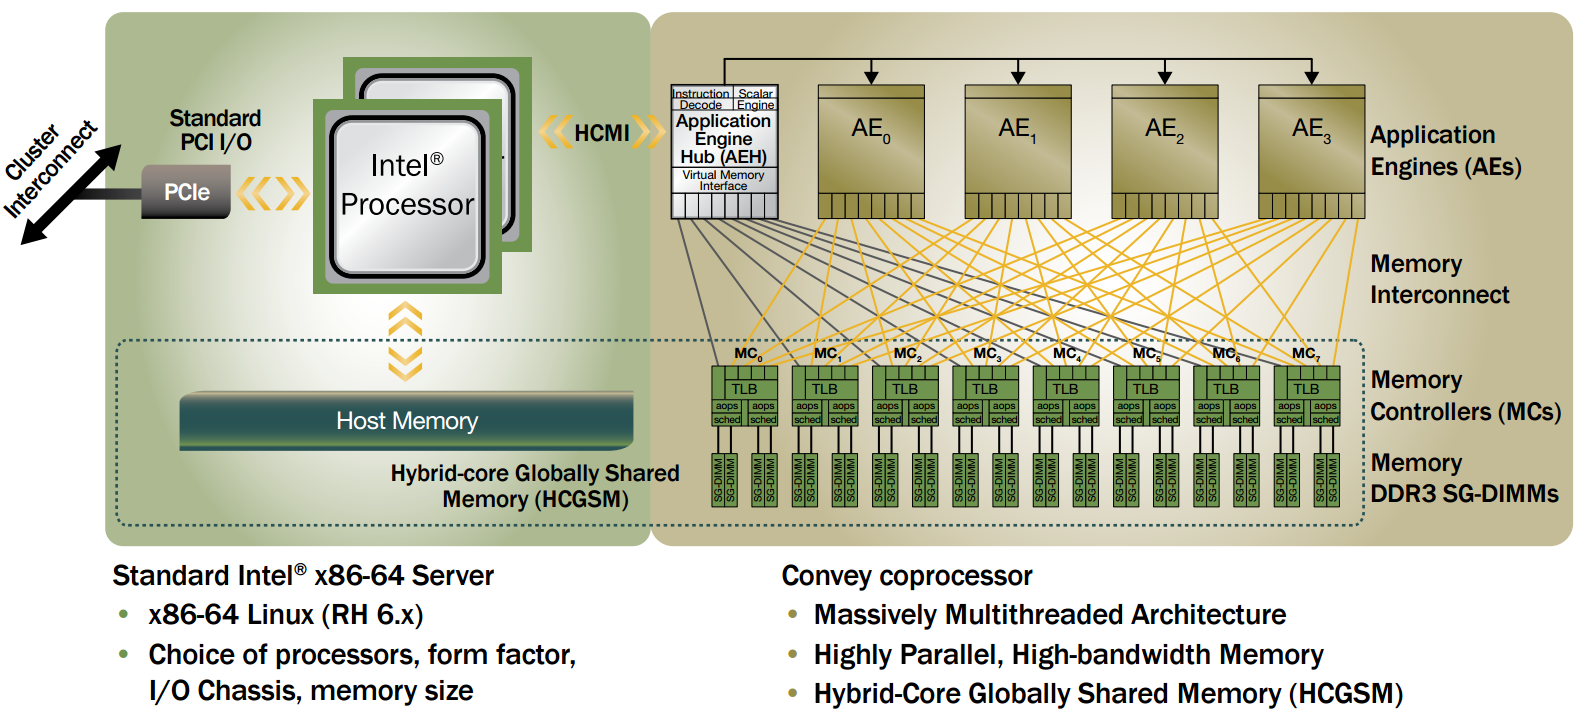
\includegraphics[width=15cm, keepaspectratio]{pics/convey.png}
\caption{Convey MX-100 architectural overview}
\label{fig:convey}
\end{figure}

I am currently targeting the Convey MX-100 as my FPGA platform. As shown in Table \ref{table:conveySpecs}, the MX-100 
is a bleeding-edge machine coupling fast general-purpose processors with multiple FPGAs with dedicated high-bandwidth 
scatter-gather memory optimized for 64-bit operations. Figure \ref{fig:convey} depicts the overall platform 
architecture. The four FPGAs, known as Application Engines, are connected with a crossbar to 8 memory controllers, 
each connecting to two channels of scatter-gather memory optimized for 64-bit random access, for a total of 16 memory 
channels. To design a Convey hybrid-core program, the engineer first designs a custom Personality, consisting of the 
FPGA bit-file containing a custom instruction set designed to accelerate individual algorithms within applications. 
The Personality source code must interface with Convey's Personality Development Kit (PDK), which presents an 
interface to Convey's abstraction layer, including its memory interface. Convey users must explicitly transfer data 
to the FPGA memory before calling the Personality instruction, and transfer the results back to CPU memory upon 
instruction completion. To run on Convey, the Galois microarchitecture resides within a Personality. The Galois HLS 
tool generates the hybrid-core program along with the required data transfers to and from FPGA memory.

The MX-100 is so far the only machine designed by Convey to support atomic memory operations, including atomic add, 
subtract, and compare-and-swap (CAS) operations. I chose the MX-100 platform because these atomic operations are 
essential for supporting high-performance synchronization across multiple FPGAs. In addition, the specialized Convey scatter-gather 
memory is perfect for supporting the pointer-chasing memory access patterns present in many Galois programs such as 
SSSP.

\subsection{Implemented Custom SSSP Engine}

\begin{figure}
\centering
\lstset{language=Java}
\begin{lstlisting}
Graph graph = { /* init */}; // Initialize graph contents
WorkList<GraphNode> workQ();
workQ.enq(init); // worklist initialized with the starting node
foreach(uint nodeId : workQ) {
   GraphNode node = graph.readNode(nodeId);
   foreach(Edge edge : graph.readEdges(node)) {
      bool retry = true;
      while(retry) {
         retry = false;
      	 uint newDist = node.dist + edge.weight;
         if(newDist < graph.readNode(edge.dest).dist) {
            if(graph.cas(node.dist, newDist)) {
               workQ.enq(edge.dest);
            }
            else {
               retry = true;
            }
         }
      }
   }
}
\end{lstlisting}
\caption{Modified Galois target code for SSSP}
\label{fig:ssspSourceCAS}
\end{figure}

\lstset{escapeinside={<@}{@>}}
\begin{figure}
\centering
\lstset{language=Java}
\begin{lstlisting}
Graph graph = { /* init */}; // Initialize graph contents
WorkList<GraphNode> workQ();
workQ.enq(init); // worklist initialized with the starting node
foreach(uint nodeId : workQ) {
   <@\textbf{\textit{graph.readNodeReq(nodeId);}}@>
   <@\textbf{\textit{GraphNode node = graph.readNodeResp();}}@>
      <@\textbf{\textit{graph.readEdgesReq(node.edgePtr + i);}}@>
      <@\textbf{\textit{foreach(Edge edge : graph.readEdgesResp());}}@>
      bool retry = true;
      while(retry) {
         retry = false;
         uint newDist = node.dist + edge.weight;
         <@\textbf{\textit{graph.readNodeReq(edge.dest);}}@>
         if(newDist < <@\textbf{\textit{graph.readNodeResp()}}@>.dist) {
            graph.casReq(node.dist, newDist);
            if(graph.casResp()) {
               workQ.enq(edge.dest);
            }
            else {
               retry = true;
            }
         }
      }
   }
}
\end{lstlisting}
\caption{Transformed Galois code for SSSP}
\label{fig:ssspSourceCASxform}
\end{figure}


\begin{figure}
\centering
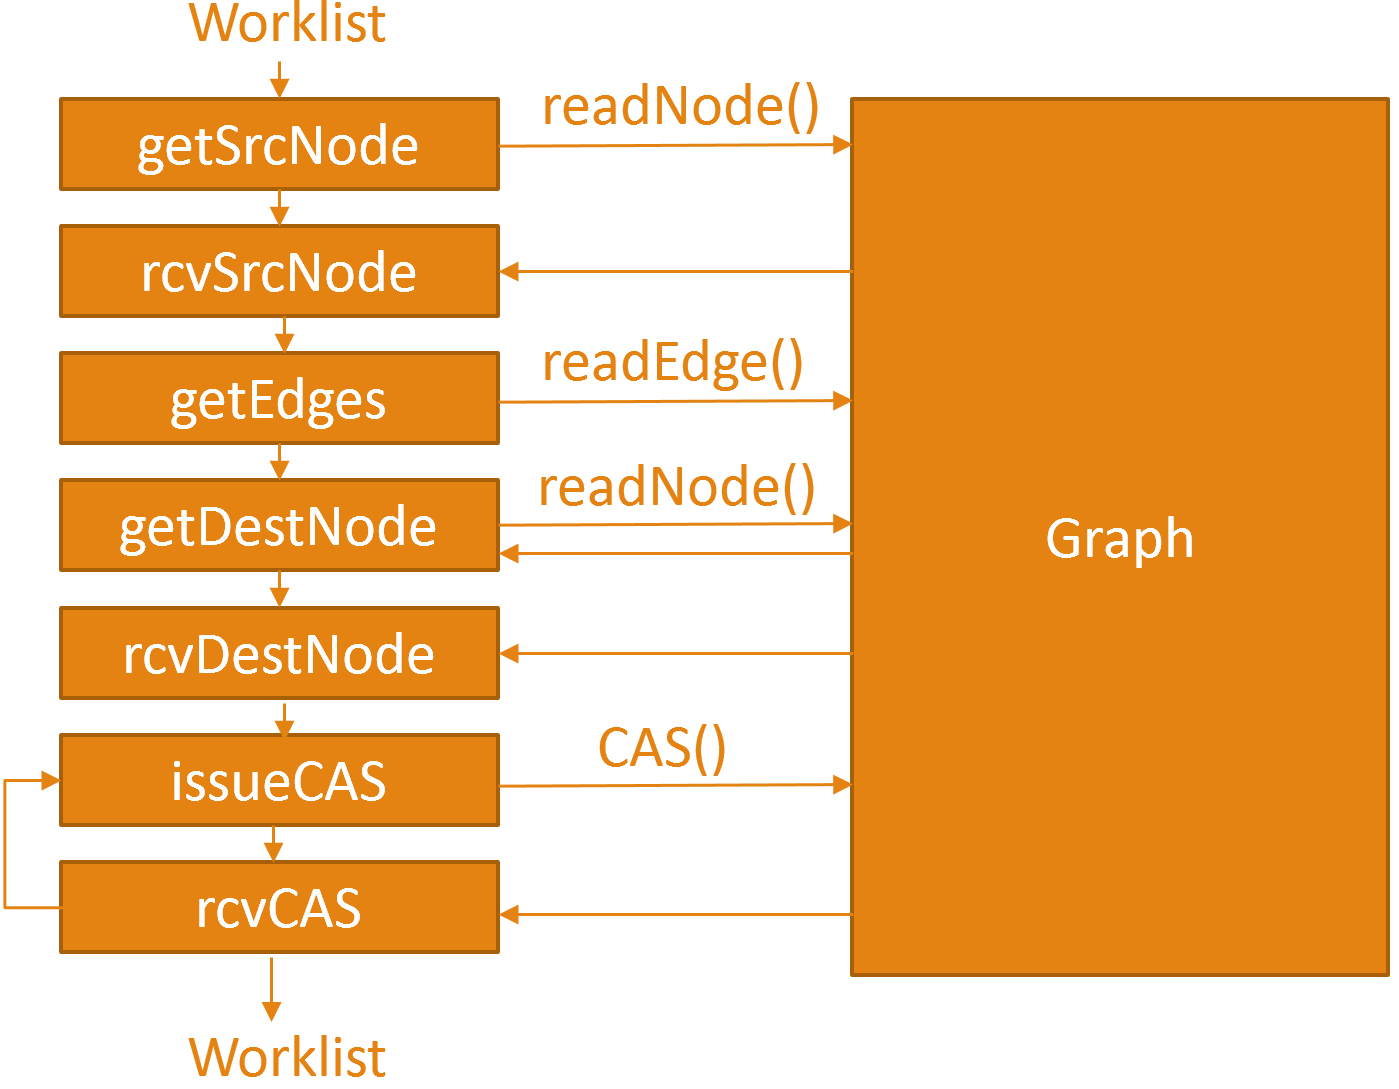
\includegraphics[width=10cm, keepaspectratio]{pics/ssspEngine.png}
\caption{Scheduled SSSP Pipeline}
\label{fig:ssspEngine}
\end{figure}

To generate the engine for SSSP, I manually performed the role of the Galois HLS compiler by scheduling the source 
code into the optimal pipeline stages and generating the requisite scaffolding. Since transactional memory support is 
in the process of being developed by my labmate Xiaoyu Ma, I chose to use a modified version of SSSP with a 
non-atomic \textbf{foreach} with explicit synchronization through the use of the atomic compare-and-swap operation. 
To maximize throughput, the compiler must support multiple Graph method calls in flight; to do this, a simple 
mechanical code transformation is necessary, shown in Figure \ref{fig:ssspSourceCASxform}. By decoupling the method 
request and response calls, the compiler can now schedule the request and response calls into different pipeline 
stages and generate the appropriate context buffering to support multiple calls in flight. The final schedule is 
shown in Figure \ref{fig:ssspEngine}, along with the decoupled Graph request and response calls.

Note that since there are loops in the pipeline, special care must be taken to prevent deadlock, which can occur when 
a thread needs to loop back but the context buffer is full. Since looping back is performed by enqueueing a thread 
context from the end of the pipeline to an earlier stage, this causes deadlock as that thread prevents other threads 
from making forward progress. I solve the deadlock issue through a credit-based system. All threads attempting to 
enter the loop must first reserve space in the context buffer. If no space exists, then the thread stalls until a 
thread has finished looping.

\subsection{Implemented Worklist}

\begin{figure}
\centering
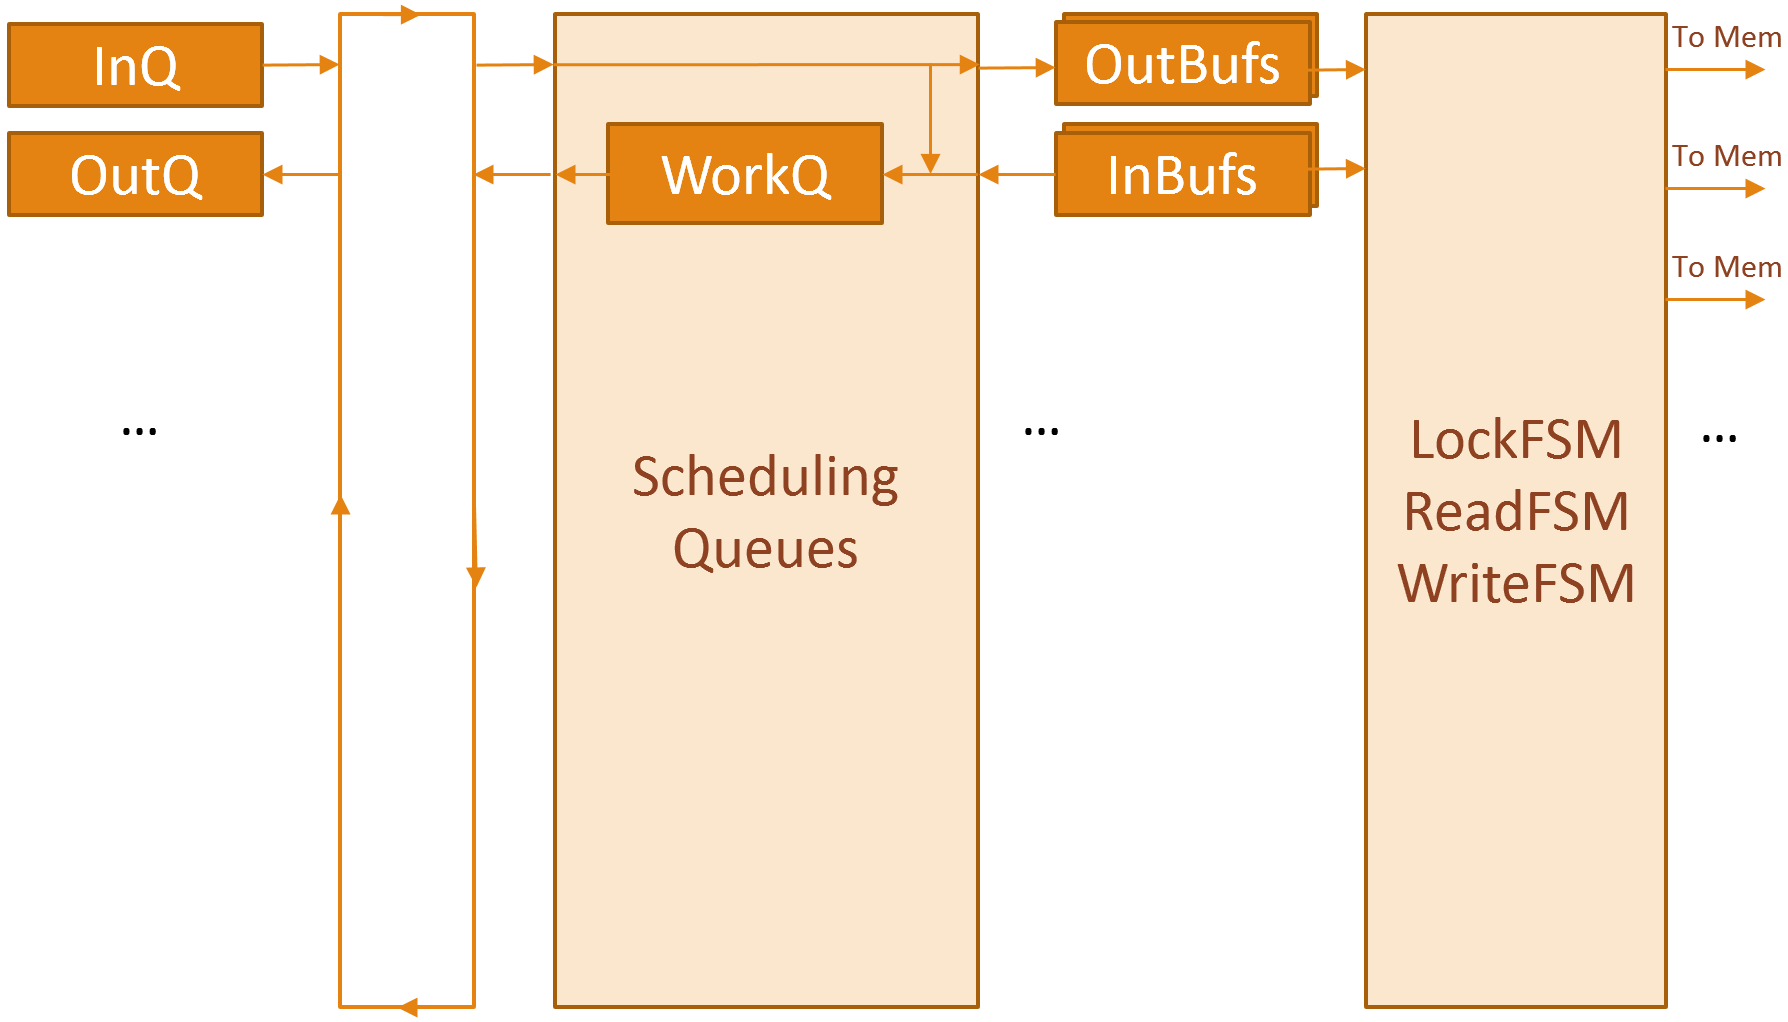
\includegraphics[width=10cm, keepaspectratio]{pics/worklist.png}
\caption{Worklist Microarchitecture}
\label{fig:worklist}
\end{figure}

\begin{figure}
\centering
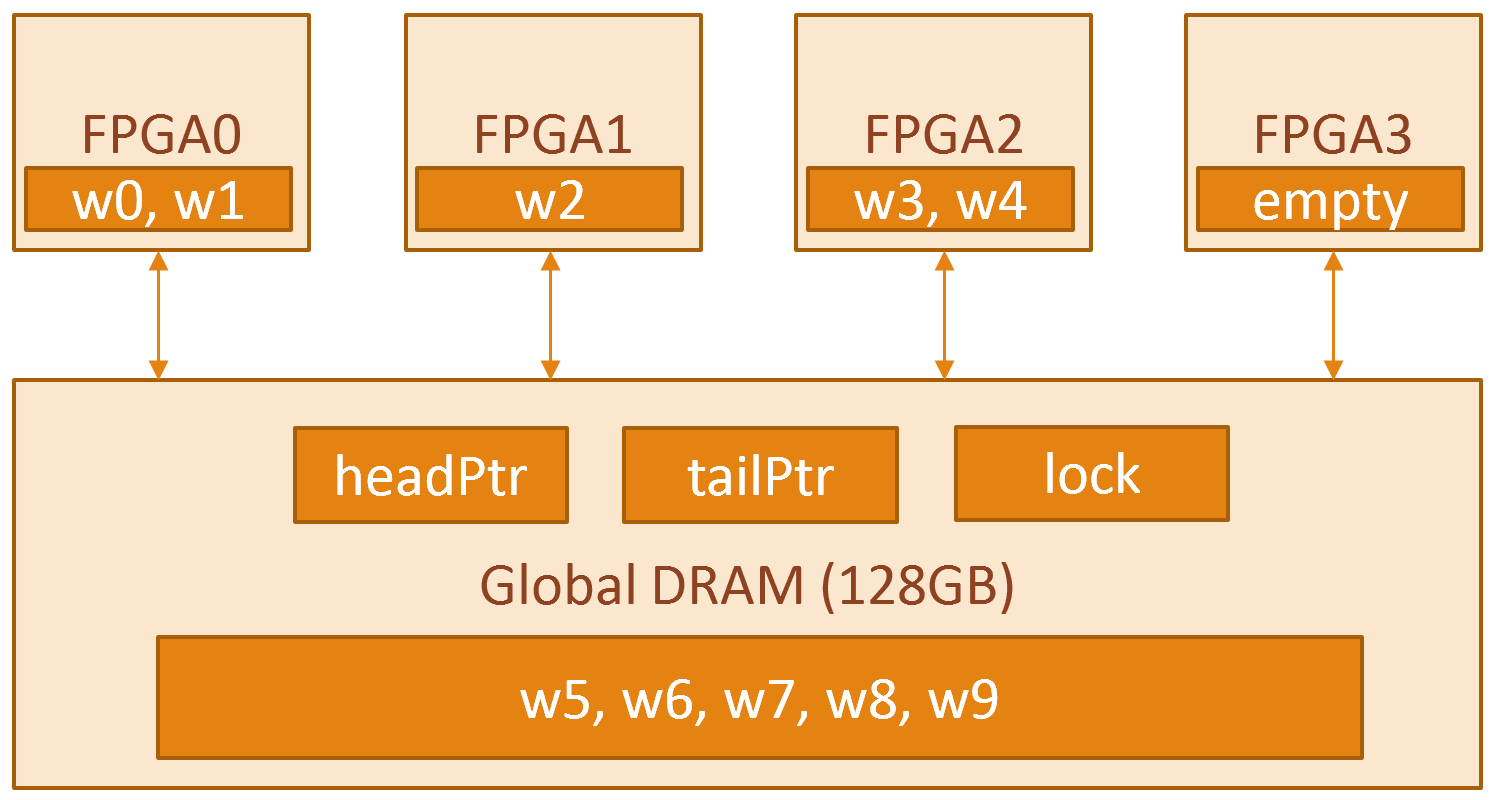
\includegraphics[width=10cm, keepaspectratio]{pics/worklistMem.png}
\caption{Worklist Data Organization Example}
\label{fig:worklistMem}
\end{figure}

For my initial worklist implementation shown in Figure \ref{fig:worklist}, I focused on designing a simple 
microarchitecture capable of scaling to a large (\~16) number of engines. The worklist is comprised of two components, 
the front-end and back-end. The front-end is responsible for work balancing across engines and implementing any 
partial priority ordering schemes specified by the user. The worklist presents a simple packet enqueue/dequeue 
interface to each engine, where each packet currently consists of a single worklist work item. The back-end handles 
worklist spills and fills to main memory.

The worklist front-end consists of \textit{N} lanes, where each lane is connected directly with the engine. Currently, 
only FIFO work ordering is supported. Each lane has a dedicated large-capacity queue (currently 2048 entries). As work 
is generated dynamically under the Galois programming model, I have implemented a work stealing ring network optimized 
for FPGA routability and fast work distribution. If an engine wishes to dequeue a worklist packet but none are 
available, the worklist sends a work steal request to its neighbor. The next time the neighbor performs a worklist 
enqueue, the packet is delivered to the requestor's work stealing queue.

When a worklist front-end lane attempts to perform an enqueue but its work queue is full, it sends the packet to the 
back-end. The back-end contains dedicated per-lane input and output double buffers to stream work items to and from 
global memory. When an output buffer is filled, the data write FSM is triggered. As shown in Figure 
\ref{fig:worklistMem}, global memory contains a unified work queue shared among all FPGAs in the system. The unified 
work queue handles work distribution between FPGAs, enables unbounded work generation, and enables each FPGA to store 
only a small percentage of work items in local BRAM. The FSM therefore locks the global unified work queue before 
writing to the queue. To minimize locking overhead, the FSM performs a streaming write operation consisting of all packets 
in a lane's output buffer (currently 1024). 

The worklist back-end read FSM is triggered when any lane's input buffers are empty and the global work queue is not 
empty. As the FPGA's worklist back-end contains a stale copy of the global worklist head and tail pointers, the 
readFSM will poll the worklist to determine if new work has been added. Like the write FSM, the read FSM locks the 
global work queue before removing entries from the queue.

\subsection{Implemented Graph}

As my labmate Xiaoyu Ma is in charge of implementing transactional memory, for the purposes of evaluating SSSP I have 
only implemented the readNode, readEdges, and compare-and-swap operations. Each operation is implemented as a pipeline 
supporting many concurrent operations in flight. Right now, as shown in Figure \ref{fig:ssspEngine}, the compiler 
instantiates a dedicated graph operation pipeline for each engine graph call. The compiler must then properly bind the 
pipeline memory requests to memory channels. With 16 engines and 16 memory channels, the compiler simply needs to map 
each engine's pipeline requests to a single memory channel. However, with 8 engines or 4 engines, the compiler must 
map more than one memory channel to a single engine's graph requests. Proper care must be taken to balance memory 
channel utilization to achieve high performance while satisfying FPGA routing constraints.


\subsection{SSSP Simulated Results}


\begin{table}
\centering
\begin{tabular}{ | l | l l | l | l | l | l |}
  \hline
  \textbf{Module} & \textbf{Slices} & \textbf{\% of total} & \textbf{Slice Reg}  & \textbf{LUTs}  & \textbf{BRAM} \\
  \hline
  XC6VHX565T & 88,560 & 100\% & 708,480 (100\%) & 354,240 (100\%) & 912 (100\%)\\
  \hline
  Convey Top & 67,586 & 76\% & 198,903 (28\%) & 182,824 (51\%) & 146 (12\%)\\
  \hline
  * BSV Wrapper & 33,979 & 38\% & 88,601 & 68,060 & 96 \\
  \hline
  ** SSSP Top & 20,831 & 24\% & 50,816 & 46,617 & 80 \\
  \hline
  *** SSSP Engines & 3,036 & 3.4\% & 8,796 & 7,916 & 24 \\
  \hline
  *** Graph & 5,576 & 6.3\% & 15,862 & 13,262 & 24 \\
  \hline
  *** Worklist & 4,491 & 5.1\% & 9,420 & 10,291 & 32 \\
  \hline
  **** Worklist Backend & 3,629 & 4.1\% & 7,650 & 8,334 & 24 \\
  \hline
\end{tabular}
\caption{SSSP FPGA Resource Usage (4 engines)}
\label{table:ssspResourceUsage}
\end{table}

\begin{table}
\centering
\begin{tabular}{ | l | l |}
  \hline
  \textbf{FPGA Count} & 4\\
  \hline
  \textbf{Engine Count per FPGA} & 4\\
  \hline
  \textbf{Clock Speed} & 125MHz\\
  \hline
  \textbf{Graph Mem Ops in Flight per Port} & 128\\
  \hline
  \textbf{Worklist Entries per Engine} & 8192\\
  \hline
  \textbf{Engine Double Buffer Size} & 1024\\
  \hline
\end{tabular}
\caption{SSSP uArch Tested Configuration}
\label{table:ssspConfig}
\end{table}

\begin{figure}
\centering
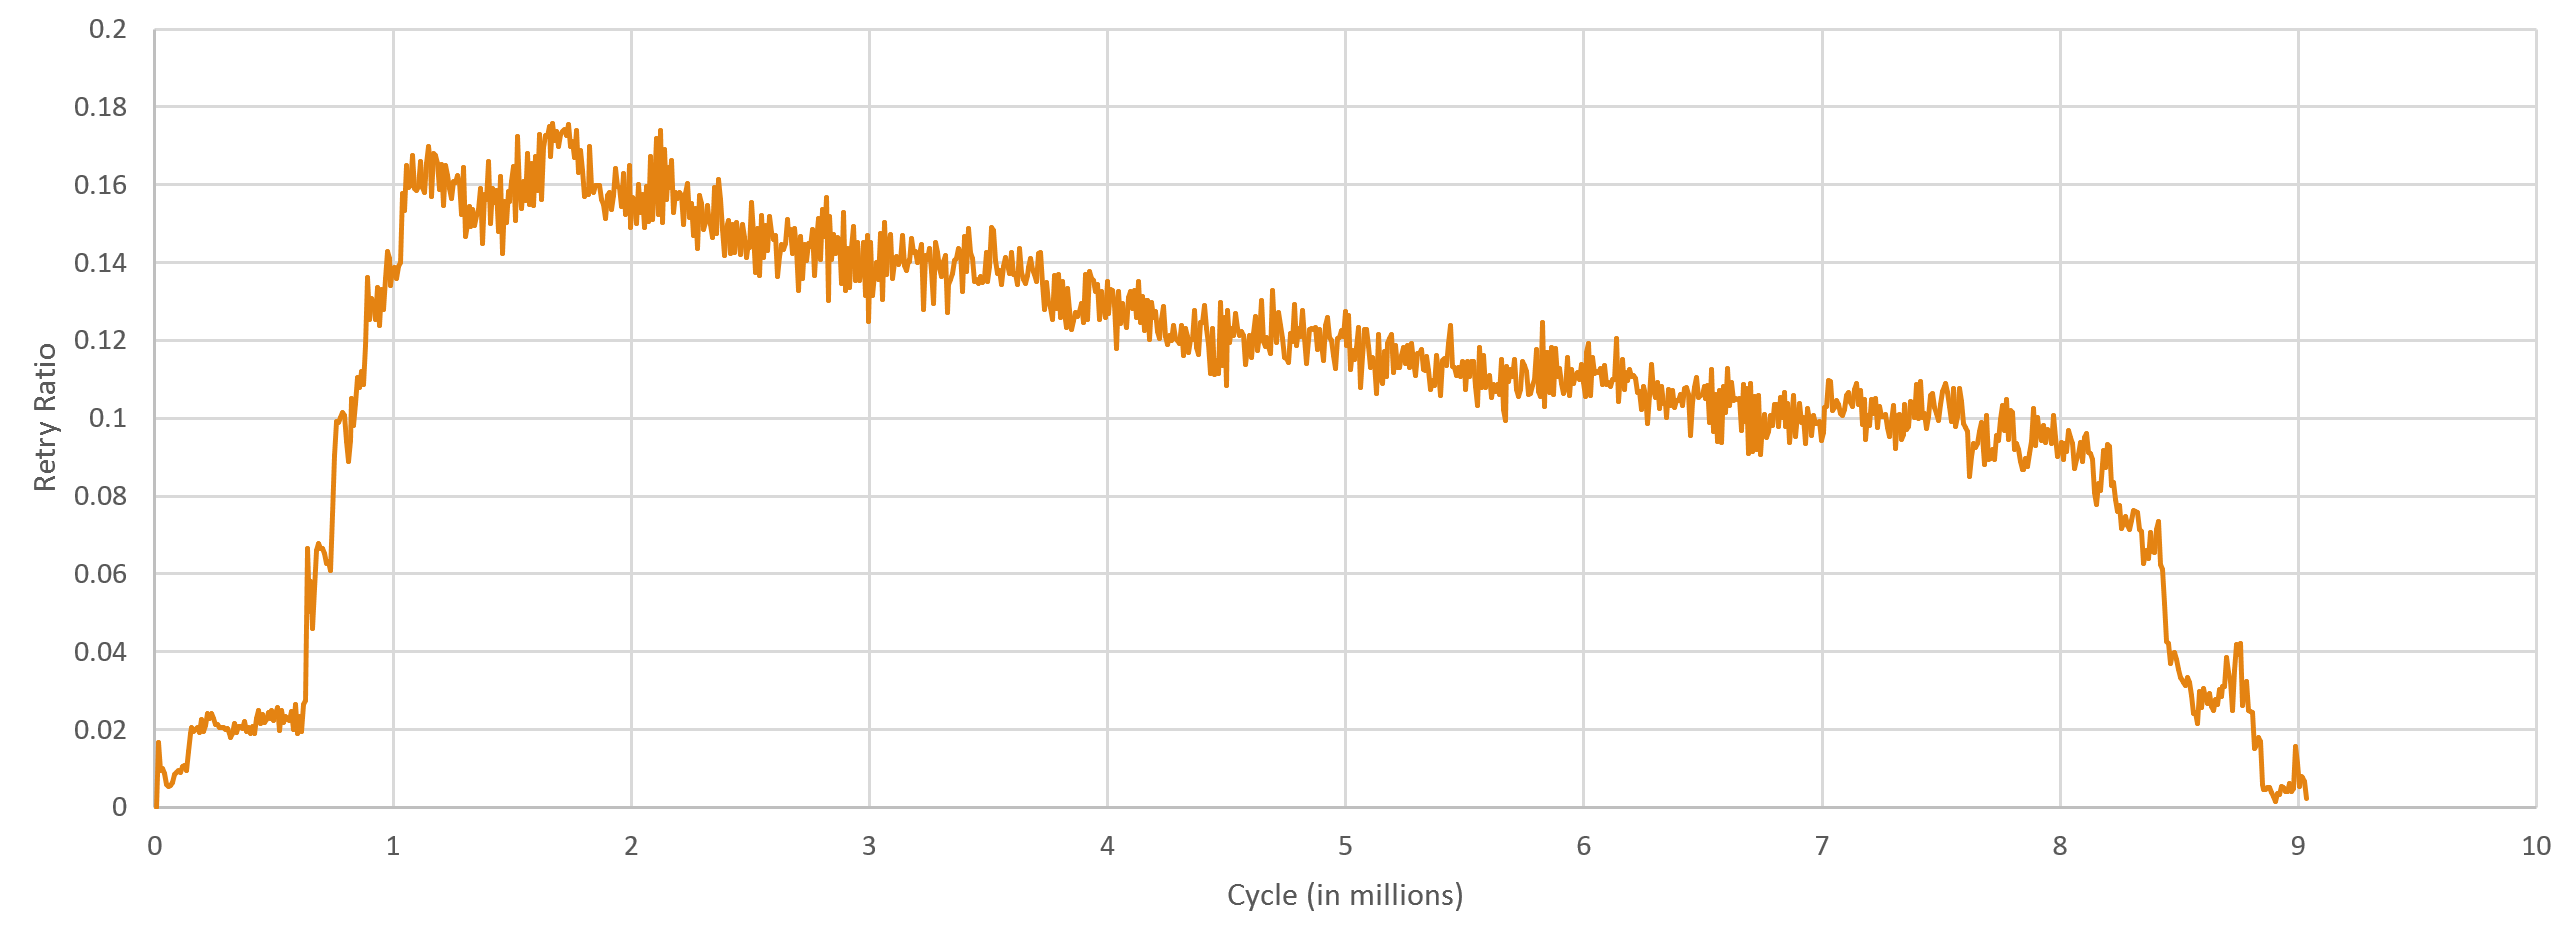
\includegraphics[width=15cm, keepaspectratio]{pics/casretry.png}
\caption{Compare-and-Swap Retry Ratio}
\label{fig:casretry}
\end{figure}

\begin{figure}
\centering
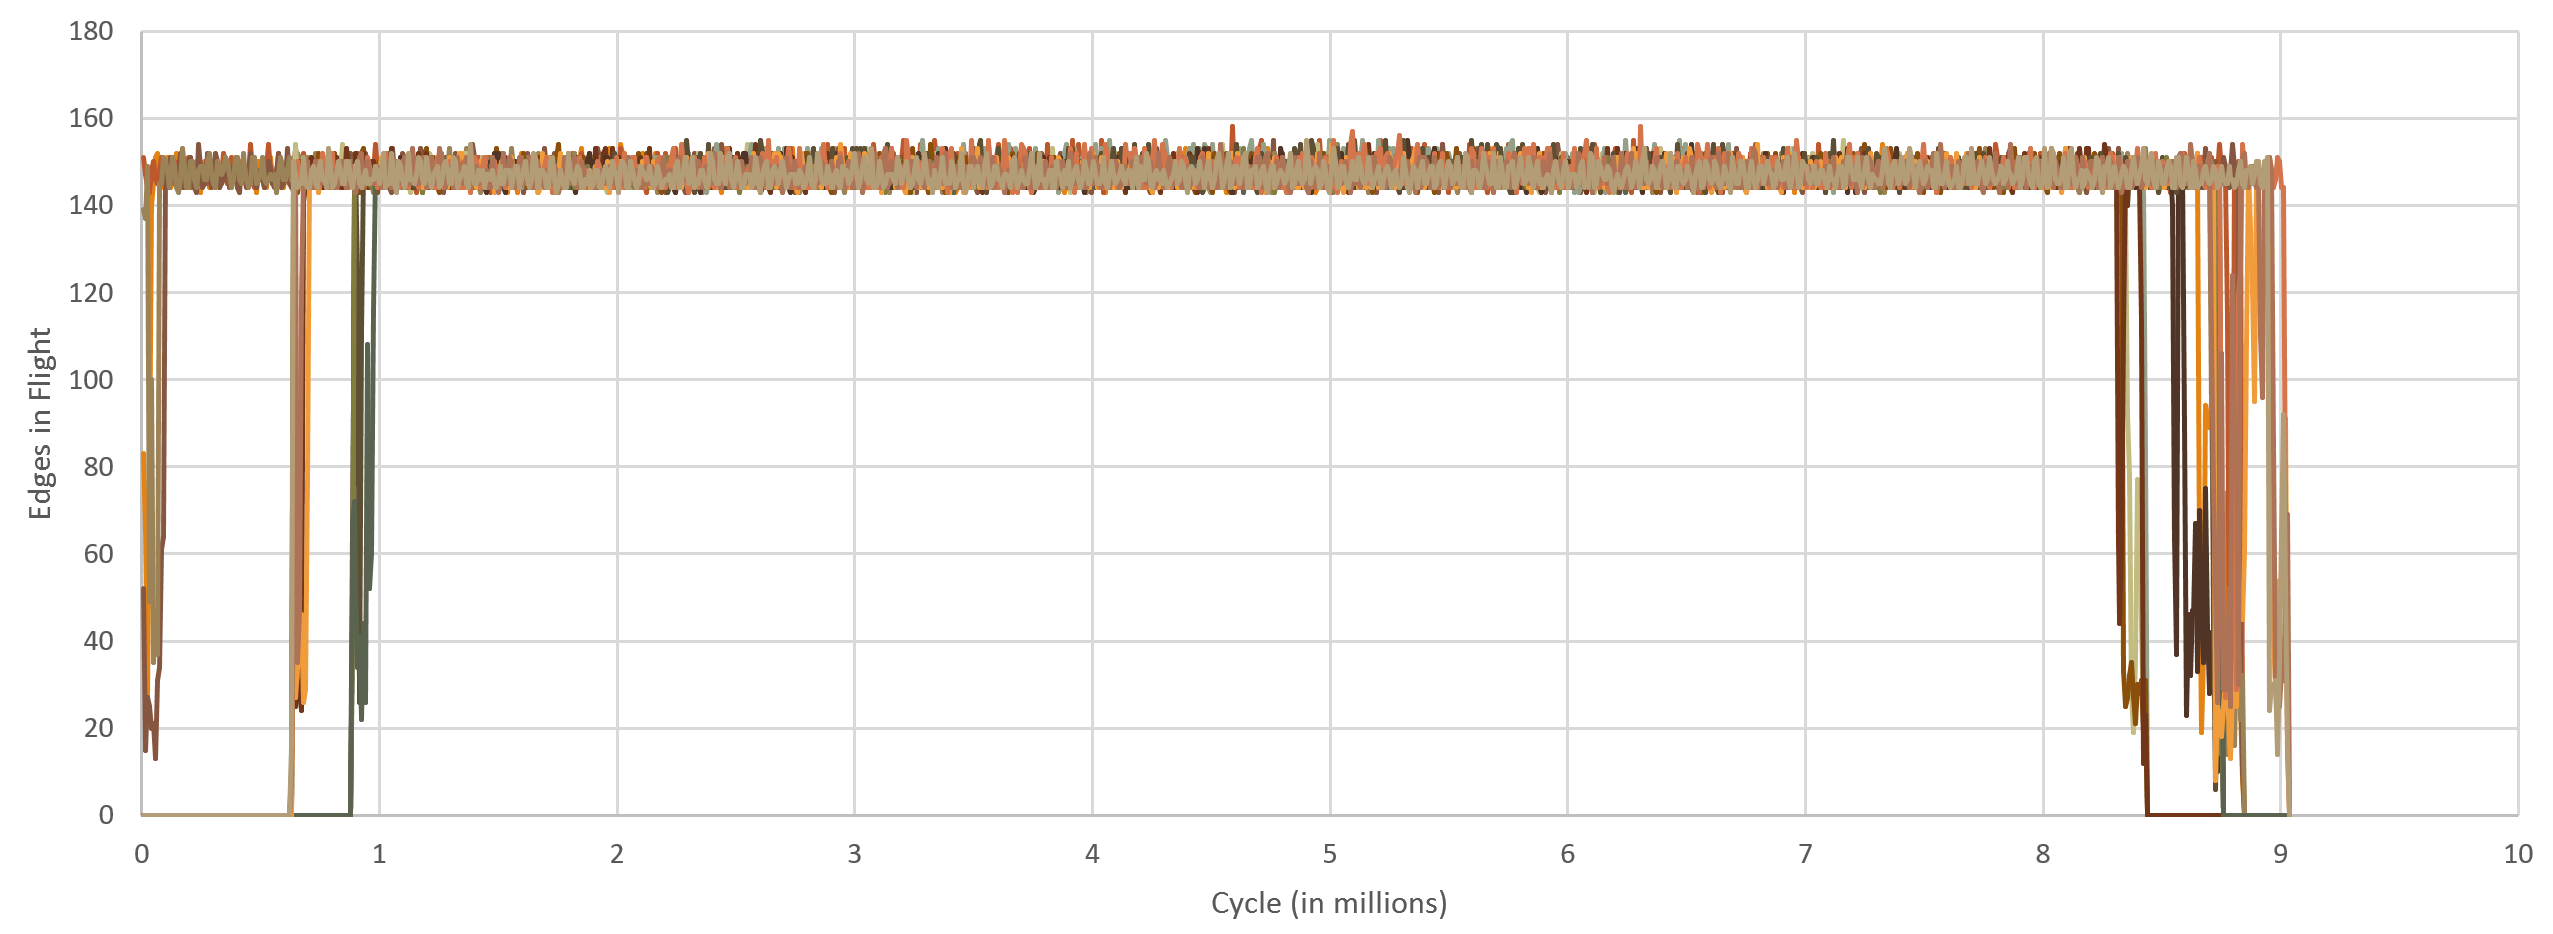
\includegraphics[width=15cm, keepaspectratio]{pics/edgesInFlight.png}
\caption{Edges in Flight per Engine}
\label{fig:edgesInFlight}
\end{figure}

\begin{figure}
\centering
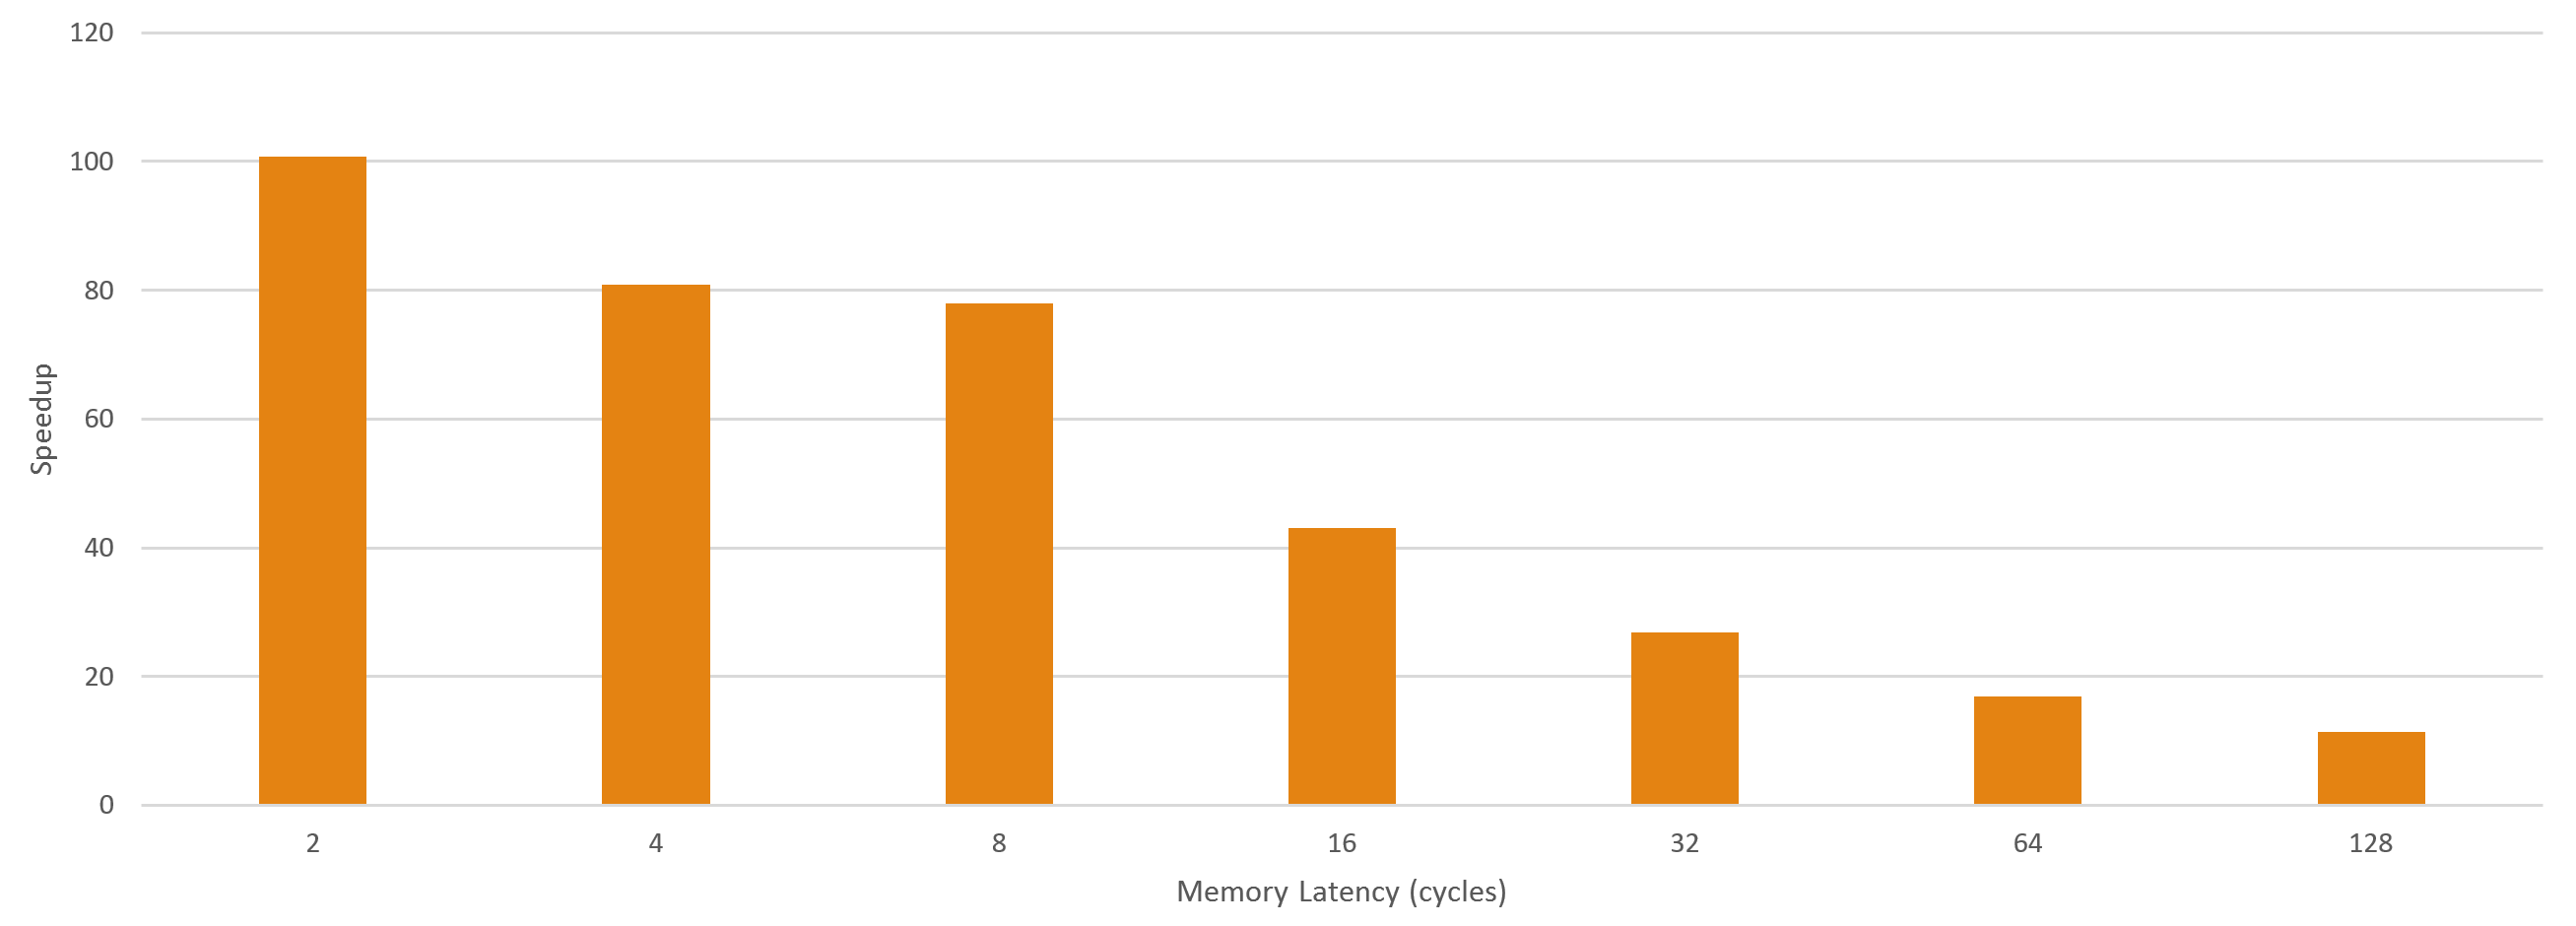
\includegraphics[width=15cm, keepaspectratio]{pics/speedup.png}
\caption{Edges Committed per Second Speedup vs. Software}
\label{fig:speedup}
\end{figure}

I was able to successfully synthesize a 4-engine SSSP microarchitecture. The FPGA bitfile is programmed to all four 
Convey Application FPGAs, resulting in 16 engines in total. The details of my configuration are shown in Table 
\ref{table:ssspConfig}. With up to 128 memory operations in flight per memory port, the design should in theory be able 
to send a memory request to each channel every cycle, resulting in up to 16 memory requests per cycle. FPGA resource 
utilization is shown in Table \ref{table:ssspResourceUsage}. Convey overheads are high: the Galois microarchitecture 
is only 32\% of the size of the entire design, consuming 24\% of total slices in the FPGA. The Bluespec wrapper itself 
uses 14\% of available FPGA slices; additional engineering effort will be required to minimize this. Unfortunately, I 
am currently unable to meet timing at 150MHz. Instead, the Galois microarchitecture is downclocked to 125MHz while 
the rest of the Convey infrastructure runs at 150MHz. 

Although I was able to synthesize my design, I have so far been unable to run on hardware due to some minor technical 
issues. However, I am able to run reasonably-sized graphs to completion in the Bluesim simulation framework. The SSSP 
design is functionally correct compared to a software golden model. For my tests, I used USA-road-NY, an undirected 
graph consisting of all roads in the state of New York, containing 264K nodes and 730K edges. However, this graph is 
too small to obtain any meaningful result running in software. As a rough approximation to overall performance, I 
measured the rate at which the SSSP engines were able to commit SSSP destination nodes. A commit occurs when a shorter 
path has been discovered, resulting in a distance update to the destination node and the destination node being added 
to the worklist. I then measured the average edges committed each second by a single-threaded Galois software 
implementation running a large workload (USA-road-USA) on a 4-socket Xeon E7540 server.

The results in Figure \ref{fig:speedup} shows the potential of the Galois microarchitecture, but also its current 
limitations. Although I can achieve 80x to 100x speedup with 2-8 cycles of memory latency, performance drops 
significantly as memory latency is swept from 16 to 128. This is due to the microarchitecture being immature; I believe 
that the issue lies with the number of memory round-trips required to synchronize and begin a worklist spill or fill 
operation. The current worklist spills to a global shared queue; a simple optimization would be to split the global 
shared queue into private queues and perform dynamic work balancing.

To preserve atomicity, SSSP node distance updates are made using the atomic compare-and-swap operation. Figure 
\ref{fig:casretry} shows the number of CAS retry operations as a function of time across the entire span of program 
execution. Retries start out low, but quickly ramp up as multiple engines are assigned work by the scheduler. The 
retry ratio peaks after all engines are warmed up and executing, and gradually decreases as each engine starts 
processing nodes further away from other engines. The small spikes near the end of execution are a result of better 
paths being discovered, resulting in idle engines being woken up and causing more conflicts.

Figure \ref{fig:edgesInFlight} shows the number of edges in flight per engine as a function of time. After each FPGA 
has been woken up, a steady state of roughly 150 edges in flight is quickly reached and remains there for the entire 
duration of program execution. This demonstrates that there is sufficient parallelism in the algorithm and input 
dataset, which enables high performance from the throughput-optimized Galois microarchitecture.

    %!TEX root = proposal.tex
% ---------------------------------------------------------------------------
\section{Research Roadmap}\label{sect:roadmap}
% ---------------------------------------------------------------------------

The preliminary SSSP Galois microarchitecture is already implemented and running within the Convey MX-100 FPGA platform 
in simulation. The remaining components of the proposed thesis and anticipated time to implement, test, and evaluate 
them are listed below:

\begin{itemize}
\item Accurate Convey MX-100 memory timing simulator to aid evaluation - 1-2 weeks.
\item Run and tune SSSP implementation on Convey MX-100 with large data inputs - 2-3 weeks.
\item Design, implement, and evaluate worklist scheduling algorithms - 4-5 months.
\item Integrate Xiaoyu Ma's transactional memory algorithms within Galois uarch - 2-4 weeks.
\item Design, implement, and evaluate HLS algorithms for engine auto-generation - 2-3 months.
\item Miscellaneous integration, tuning, testing, and debugging - 1-2 months.
\item Writing of dissertation and preparing for thesis defense - 2 months.
\end{itemize}

In total, I anticipate roughly 12 to 15 months of work remain to complete the proposed work, 
produce the dissertation, and prepare for the thesis defense.


    %!TEX root = proposal.tex
% ---------------------------------------------------------------------------
\section{Conclusion}\label{sect:conclusion}
% ---------------------------------------------------------------------------
I propose the use of the parallel graph language Galois for FPGA, which presents a high-level transactional programming 
model, allowing the user to describe the fine-grained task parallelism available in amorphous data-parallel graph algorithms to be more easily 
extracted by the compiler and Galois runtime. By combining the high-level transactional semantics of Galois with 
the automatic Galois HLS compiler and Galois microarchitecture that supports dynamic scheduling and synchronization, my tool can simultaneously improve 
quality of results while decreasing programmer effort. To achieve these goals, I will augment an existing HLS compiler 
to support the Galois unordered \textbf{foreach} loop iterator, and design a set of Galois library components and 
Galois microarchitectural template. The compiler will emit custom pipelined engines and connect them to my proposed Galois 
microarchitecture. Given the scope of the project, I will first focus on Galois programs that do not modify the structure of 
the input graph, but will later experiment with a simple memory allocator for mutable graphs. 
I will also not be focusing on preserving atomicity across \textbf{foreach} loop iterations, as that 
is the thesis project of my labmate Xiaoyu Ma. Preliminary results for SSSP demonstrate that my proposed Galois 
microarchitecture is promising and should be effective for accelerating other Galois programs.




%   ==========================================================================
%   Wrap up the document with the Bibliography (looks for the specified .bib)
%   ==========================================================================
    \makebibliography{bibliography}
\end{document}
